The system consists of two parts, one that is designed to run in real-time on a laptop or other mid-end processing device, complete with GUI for debugging and parameter tuning. An other, more slim version designed to run, in real-time on a Raspberry Pi\footnote{The words "Raspberry Pi" and the Raspberry Pi logo are trademarks of the Raspberry Pi Foundation} computer configuration, with a Raspberry-Pi cameras is also delivered. In the former case all processing of data takes place on the processing unit and is presented to the user via the debug-GUI. The Raspberry Pi-system, image processing is performed locally on the board with information about people entering/exiting being transmitted via Ethernet to receiving device. Below is an overview of the system.

\vspace{0.5cm}
\begin{figure}[htb]
	\centering
	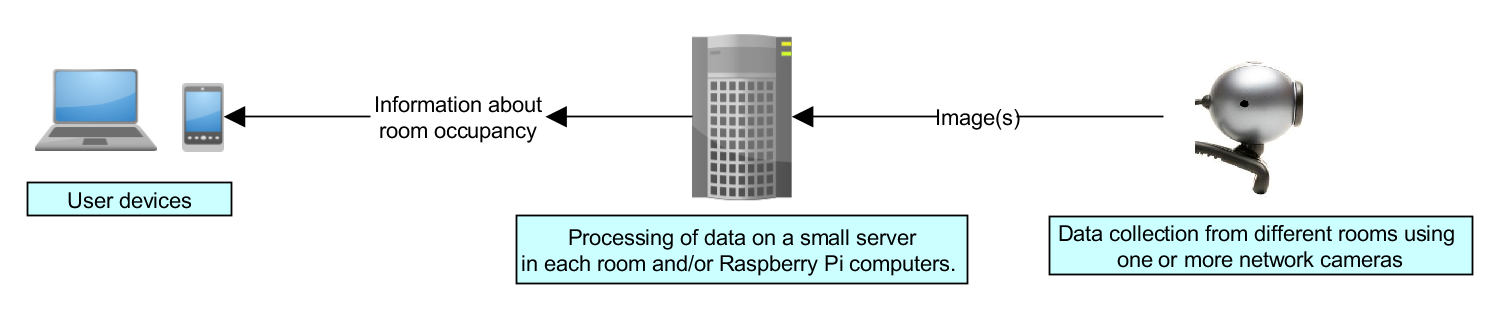
\includegraphics[width=170mm]{images/system_overview.png}
	\caption[System overview]{\textit{A simplified overview of the system}}
	\label{fig:block_overview2_fig}  %Skapar referens till figuren
\end{figure}

\subsection{Rough description of the systems}
The camera(s) used to collect data are connected to the processing unit via Ethernet, or USB in case where one processing unit per room is used. For integrity reasons, the network connecting the cameras to the local processing unit needs to be private and through cable. For the Raspberry Pi system, a special Raspberry-Pi camera board, or a Microsoft Kinect is used. The main program collects data from the cameras in a room to perform an estimation of room usage intensity, which is then presented to the user in an understandable format, e.g. estimated waiting time or current amount of people in the room.
\newpage
\subsection{Components}
The main components of the system are the cameras, the image processing unit(s), and the result presentation page.

\subsubsection{Hardware}
The system runs on both Raspberry Pis and a regular laptop. The laptop system runs on any OpenCV-compatible camera as well as the Microsoft Kinect, whereas the Raspberry Pi system requires the Raspberry Pi camera board as an input. For a more detailed description of the hardware requirements, see section \ref{sec:hardware}.

\subsubsection{Software}
In the case of regular cameras being used, the software will be running on a server where both image processing, estimation of queue size and waiting time takes place. If the Raspberry Pi:s are used, image processing takes place locally on each board. For a more thorough description of the image processing and estimation programs, see section \ref{sec:software}.

\subsection{Usability and installation}
In order to create a system that is cheap to use and install, it needs to be easy to set up, which is why a user's manual and an installation/calibration program is provided with the system if necessary. As for the usability, relevant data is presented to the user on a web page or via the Debug-GUI in case of further development (see section \ref{sec:usage}). 

